% Graphical abstract for the paper.
%
% Elsevier / EMS constraints honoured here:
%   * canvas ~166 x 66 mm (2.5:1); >= 1328 x 531 px at 300 dpi
%   * fonts restricted to Times (math), Helvetica/Arial (text), Courier (code)
%   * no title, no synopsis block, no padding, no "Graphical Abstract" label
%   * one left-to-right forward path, one return path
%   * hierarchy carried by stroke weight, so the figure survives grayscale
%   * colour is reserved for the rate-expression token kinds (Figure 2 palette);
%     the process units are neutral, so no hue is decorative
%
% The model card is literal, loadable aquakin: the excerpt parses through
% load_model_from_file and its rate evaluates to muH*[SS]/(KS+[SS])*[XB_H].
%
% Build:  latexmk -pdf graphical_abstract.tex
%
\documentclass[border=1pt]{standalone}

\usepackage[T1]{fontenc}
\usepackage{mathptmx}                       % Times, for math
\usepackage{helvet}                         % Helvetica (Arial), for text
\usepackage{courier}                        % Courier, for the model file
\usepackage{bm}
\renewcommand{\familydefault}{\sfdefault}

\usepackage{tikz}
\usetikzlibrary{positioning,arrows.meta,calc}

% Token palette carried over from Figure 2 of the manuscript. Teal/amber/violet
% is colourblind-safe, and the notation is redundant with the colour: a species
% wears brackets, a function wears parentheses. The figure reads in grayscale.
\definecolor{rlspec}{HTML}{0B7A75}
\definecolor{rlparam}{HTML}{B26A00}
\definecolor{rlfunc}{HTML}{7B3FA0}
\definecolor{yamlkey}{HTML}{1A4789}

\newcommand{\kw}[1]{\textcolor{yamlkey}{\textbf{#1}}}
\newcommand{\sptok}[1]{\textcolor{rlspec}{#1}}
\newcommand{\partok}[1]{\textcolor{rlparam}{#1}}
\newcommand{\fntok}[1]{\textcolor{rlfunc}{#1}}
\newcommand{\qt}[1]{\textcolor{black!45}{#1}}

\begin{document}
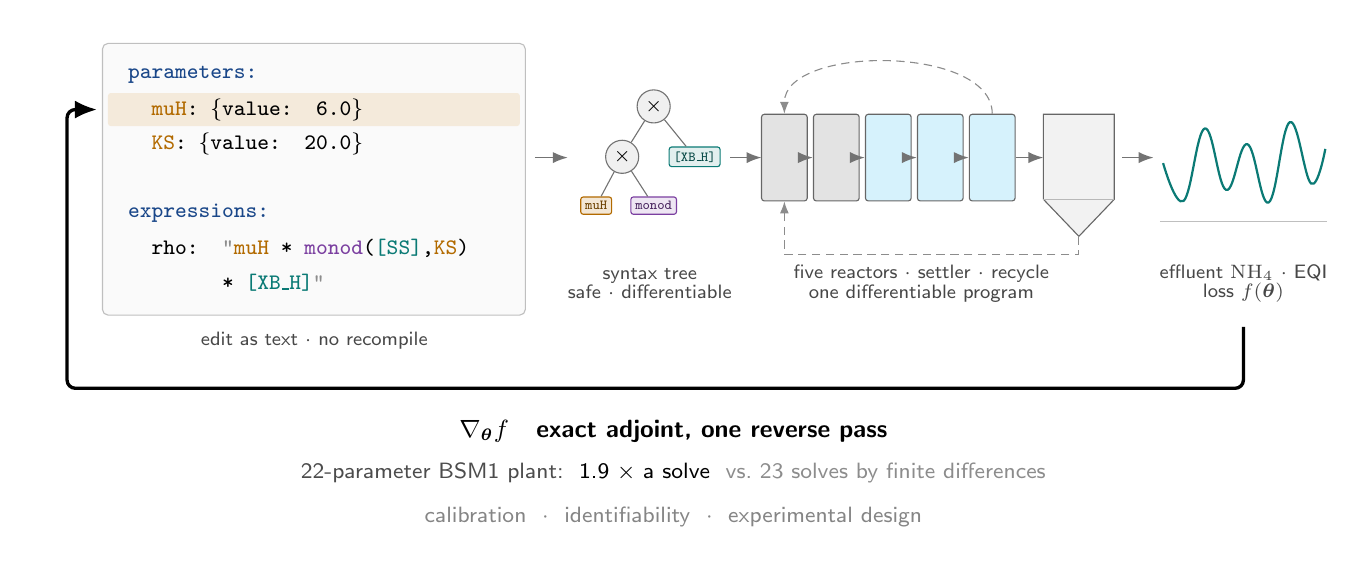
\begin{tikzpicture}[
    x=1cm, y=1cm,
    yml/.style={anchor=west, font=\ttfamily\footnotesize},
    fwd/.style={->, >={Latex[length=1.9mm]}, draw=black!55, semithick},
    tank/.style={draw=black!60, rounded corners=1pt, minimum width=0.58cm,
                 minimum height=1.10cm, inner sep=0pt},
    anox/.style={tank, fill=black!11},
    aer/.style={tank, fill=cyan!16},
    recyc/.style={->, >={Latex[length=1.5mm]}, densely dashed, draw=black!45, thin},
    lbl/.style={font=\scriptsize, text=black!72, align=center},
  ]

  \useasboundingbox (0,0) rectangle (16.6,6.60);

  % =====================================================================
  % ZONE A -- the model as data
  % =====================================================================
  \fill[black!2, rounded corners=2pt] (0.95,2.95) rectangle (6.32,6.40);
  \draw[black!25, rounded corners=2pt] (0.95,2.95) rectangle (6.32,6.40);

  % The parameter that the return arrow lands on.
  \fill[rlparam!14, rounded corners=1pt] (1.02,5.35) rectangle (6.25,5.77);

  \node[yml] at (1.15,6.00) {\kw{parameters:}};
  \node[yml] at (1.15,5.56) {\ \ \partok{muH}: \{value: 6.0\}};
  \node[yml] at (1.15,5.12) {\ \ \partok{KS}:\ \{value: 20.0\}};
  \node[yml] at (1.15,4.24) {\kw{expressions:}};
  \node[yml] at (1.15,3.80) {\ \ rho: \qt{"}\partok{muH} * \fntok{monod}(\sptok{[SS]},\partok{KS})};
  \node[yml] at (1.15,3.36) {\ \ \ \ \ \ \ \ * \sptok{[XB\_H]}\qt{"}};

  \node[lbl] at (3.64,2.62) {edit as text $\cdot$ no recompile};

  % =====================================================================
  % ZONE B -- parsed to a syntax tree
  % =====================================================================
  \draw[fwd] (6.44,4.95) -- (6.86,4.95);

  \begin{scope}[
      op/.style={draw=black!55, circle, inner sep=0.5pt, fill=black!6,
                 minimum size=4.2mm, font=\scriptsize},
      lf/.style={rounded corners=0.9pt, inner sep=1.6pt, font=\ttfamily\tiny}]
    \node[op] (m1) at (7.95,5.60) {$\times$};
    \node[op] (m2) at (7.55,4.96) {$\times$};
    \node[lf, draw=rlspec, fill=rlspec!12, text=rlspec!60!black]
         (xh) at (8.47,4.96) {[XB\_H]};
    \node[lf, draw=rlparam, fill=rlparam!16, text=rlparam!60!black]
         (mu) at (7.22,4.34) {muH};
    \node[lf, draw=rlfunc, fill=rlfunc!13, text=rlfunc!60!black]
         (mo) at (7.95,4.34) {monod};
    \draw[black!55, thin] (m1) -- (m2);
    \draw[black!55, thin] (m1) -- (xh);
    \draw[black!55, thin] (m2) -- (mu);
    \draw[black!55, thin] (m2) -- (mo);
  \end{scope}

  \node[lbl] at (7.90,3.35) {syntax tree\\[-1pt] safe $\cdot$ differentiable};

  \draw[fwd] (8.92,4.95) -- (9.32,4.95);

  % =====================================================================
  % ZONE C -- one differentiable program
  % =====================================================================
  \node[anox] (t1) at (9.61,4.95) {};
  \node[anox] (t2) at (10.27,4.95) {};
  \node[aer]  (t3) at (10.93,4.95) {};
  \node[aer]  (t4) at (11.59,4.95) {};
  \node[aer]  (t5) at (12.25,4.95) {};

  % Secondary clarifier: rectangular body over a sludge hopper.
  \fill[black!5] (12.90,5.50) -- (13.80,5.50) -- (13.80,4.42) --
                 (13.35,3.95) -- (12.90,4.42) -- cycle;
  \draw[black!60] (12.90,5.50) -- (13.80,5.50) -- (13.80,4.42) --
                  (13.35,3.95) -- (12.90,4.42) -- cycle;
  \draw[black!28, thin] (12.90,4.42) -- (13.80,4.42);

  \foreach \a/\b in {t1/t2, t2/t3, t3/t4, t4/t5} {\draw[fwd] (\a) -- (\b);}
  \draw[fwd] (t5.east) -- (12.90,4.95);

  \draw[recyc] (t5.north) to[out=90,in=90,looseness=0.85] (t1.north);
  \draw[recyc] (13.35,3.95) -- (13.35,3.72) -- (9.61,3.72) -- (t1.south);

  \node[lbl] at (11.35,3.35)
       {five reactors $\cdot$ settler $\cdot$ recycle\\[-1pt]
        one differentiable program};

  % =====================================================================
  % ZONE D -- the output
  % =====================================================================
  \draw[fwd] (13.90,4.95) -- (14.30,4.95);

  \draw[black!25, thin] (14.38,4.14) -- (16.50,4.14);
  \draw[rlspec, thick] plot[smooth, tension=0.7] coordinates {
    (14.42,4.88) (14.68,4.40) (14.95,5.32) (15.22,4.54)
    (15.49,5.12) (15.76,4.38) (16.03,5.40) (16.30,4.62) (16.48,5.06)};

  \node[lbl] at (15.44,3.35)
       {effluent $\mathrm{NH_4}$ $\cdot$ EQI\\[-1pt] loss $f(\bm{\theta})$};

  % =====================================================================
  % THE RETURN PATH -- the heaviest ink on the canvas.
  % It leaves the output, sweeps beneath the whole figure, and terminates on
  % the parameter in the text file. The same gesture as the plant's own
  % return-sludge line, one level up: it carries derivatives, not sludge.
  % =====================================================================
  \draw[line width=1.2pt, draw=black, >={Latex[length=2.8mm, width=2.3mm]}, ->,
        rounded corners=3pt]
    (15.44,2.80) -- (15.44,2.02) -- (0.50,2.02) -- (0.50,5.56) -- (0.88,5.56);

  \node[font=\small\bfseries, text=black] at (8.20,1.48)
       {$\nabla_{\bm{\theta}} f$ \ \ exact adjoint, one reverse pass};
  \node[font=\footnotesize] at (8.20,0.94)
       {\textcolor{black!70}{22-parameter BSM1 plant:}\ \
        \textcolor{black}{1.9 $\times$ a solve}\ \
        \textcolor{black!45}{vs.\ 23 solves by finite differences}};
  \node[font=\footnotesize, text=black!48] at (8.20,0.38)
       {calibration $\ \cdot\ $ identifiability $\ \cdot\ $ experimental design};

\end{tikzpicture}
\end{document}
